\section{Methodology}\label{section:methodology}

\lettrine{T}{he} prospective solution was ultimately named \emph{Packet Courier} for reasons that the ensuing design
documentation aims to make clear. In summary, Packet Courier listens for packets being sent by nodes on its virtual
network, processing and rerouting them according to their listed destination and the associated conditions; just as a
mail courier would do analogously for letters and parcels. The metaphor also aligns itself well with the overall
motivations of the project, whereby postal services are largely seen as reliable infrastructure that operate silently
in the background, enabling people to send goods across seemingly vast distances without needing to worry about how
this is achieved. Indeed, these are the ideals that Packet Courier strives to embody, especially in light of
objectives 4) and 5).

Packet Courier has been designed and developed by leveraging philosophies from the \emph{lean development} school of
thought\cite{william_feld_lean_book, steve_blank_lean_blog}. This involved making Packet Courier a functional and
useful piece of software from the very first iteration, and continuing to ensure that this remained so with each new
feature. As a consequence, every supervisory meeting, informal peer review or user ``playtest'' would be a
meaningfully different experience, with something novel to demonstrate on each occasion. In this way, any feedback
could be readily taken on-board and implemented quickly. By contrast, if Packet Courier had been meticulously
designed from the bottom-up or the top-down, even the smallest changes in direction could risk rendering much of the
planning totally obsolete.

The simplest way to guarantee that Packet Courier provided users with tangible value from day one was to integrate an
application-programmer interface into the base simulation engine. That way, developers could always take advantage of
what Packet Courier had to offer, even if it was primitive. This ended up paying dividends down-the-line, as it was this
combination of design philosophy and system architecture that facilitated the development of Packet Courier's
emulation mode, which leveraged the base simulation APIs to further empower Packet Courier to manipulate authentic
UDP packets in real-time.


\section{High-Level Architecture}\label{section:high_level_architecture}

\subsection{Simulation Semantics}\label{subsection:simulation_semantics}

\lettrine{M}{any} of Packet Courier's core abstractions are inspired by the Elixir programming language\cite{elixir}.
One of Elixir's major selling points is how elegantly it removes unnecessary detail when interfacing with the
programmer. Rather than hemming developers into considering bits being sent over a wire, or packets being sent over a
network, Elixir talks in terms of \emph{processes} exchanging \emph{messages} with one
another\cite{elixir_processes}, which could consist of any high-level object such as text, numbers, tuples, or even
higher-order structures like lists and structs. Furthermore, Elixir uses neat allegories to help developers build up
a more intuitive picture of what their code does, i.e.: collecting messages from a \emph{mailbox} or using an
arbitrary \emph{process-id} rather than an ip-address. Not only does this improve readability, but it also insulates
the logic of the distributed algorithms from the lower-level details of the machine or the network. Is \texttt{ipv4}
or \texttt{ipv6} being used? An Elixir developer wouldn't need to know or care.

As such, Packet Courier channels Elixir's spirit of using intuitive, high-level concepts to help users quickly build
an understanding for a given simulation. As one might expect, the \emph{Node} is a cornerstone abstraction within the
Packet Courier framework. A node represents a particular location within a wider network topology and enjoys a unique
\emph{Node Address}. Each node will have at least one \emph{Worker}, where each worker will in turn carry out some
work in the form of a coroutine. Workers also have access to a \emph{Postal Service} which enables them to interact
with the wider network by sending a \emph{Packet} to a destination \emph{WorkerAddress}. The postal service will then
package the packet and destination worker address into a single piece of \emph{Mail} and send it along the
\emph{Node Connection} associated with the source and destination worker addresses (provided it exists). Notice that
the mail is sent along a node connection, as opposed to a \emph{worker} connection, because mail is principally
exchanged between nodes rather than workers. In this way, when a piece of mail arrives at its destination node, the
node extracts and routes the packet to its respective worker address; idiomatically speaking, the node
\emph{Delivers} the packet to the worker's \emph{Mailbox}. The worker then has the option to poll packets from its
mailbox. It is important to note that mailboxes store packets, not \emph{mail}. The rationale behind this is that one
needn't accompany their letter or parcel with a return address in order to send it; this is a choice that can be made
at the sender's discretion. Workers are also granted privacy, meaning that they can only see the contents of their own
mailbox.

Drilling down into the specifics of packet transmission, each node connection is associated with a \emph{Packet
Pipeline}. As the name suggests, a packet pipeline is a linear conduit whereby packets are processed in a fashion
akin to a conveyor-belt, and it is herein that any packet manipulation is conducted, i.e.: latency, drop, corruption.
The nature of this architecture is the first reason why packet communication occurs between nodes and not workers. If
$n$ nodes had on average $w$ workers each, then the maximum number of unidirectional inter-node connections would be
$n(n-1)$, yet the expected number of unidirectional inter-worker connections would be $w^2n(n-1)$. Thus, it is much
more resource efficient for the workers to simply delegate mail sorting responsibilities to their respective node. In
addition, workers are temporal insofar as they can be added and removed from the simulation dynamically like threads,
which would mean that packet pipelines would need to be introduced on-the-fly in a way that would only mirror
node-to-node semantics anyway, since workers inherit their position in the topology (i.e.: who they can send packets
to and with what network conditions) from their node.

\begin{figure}[!h]
    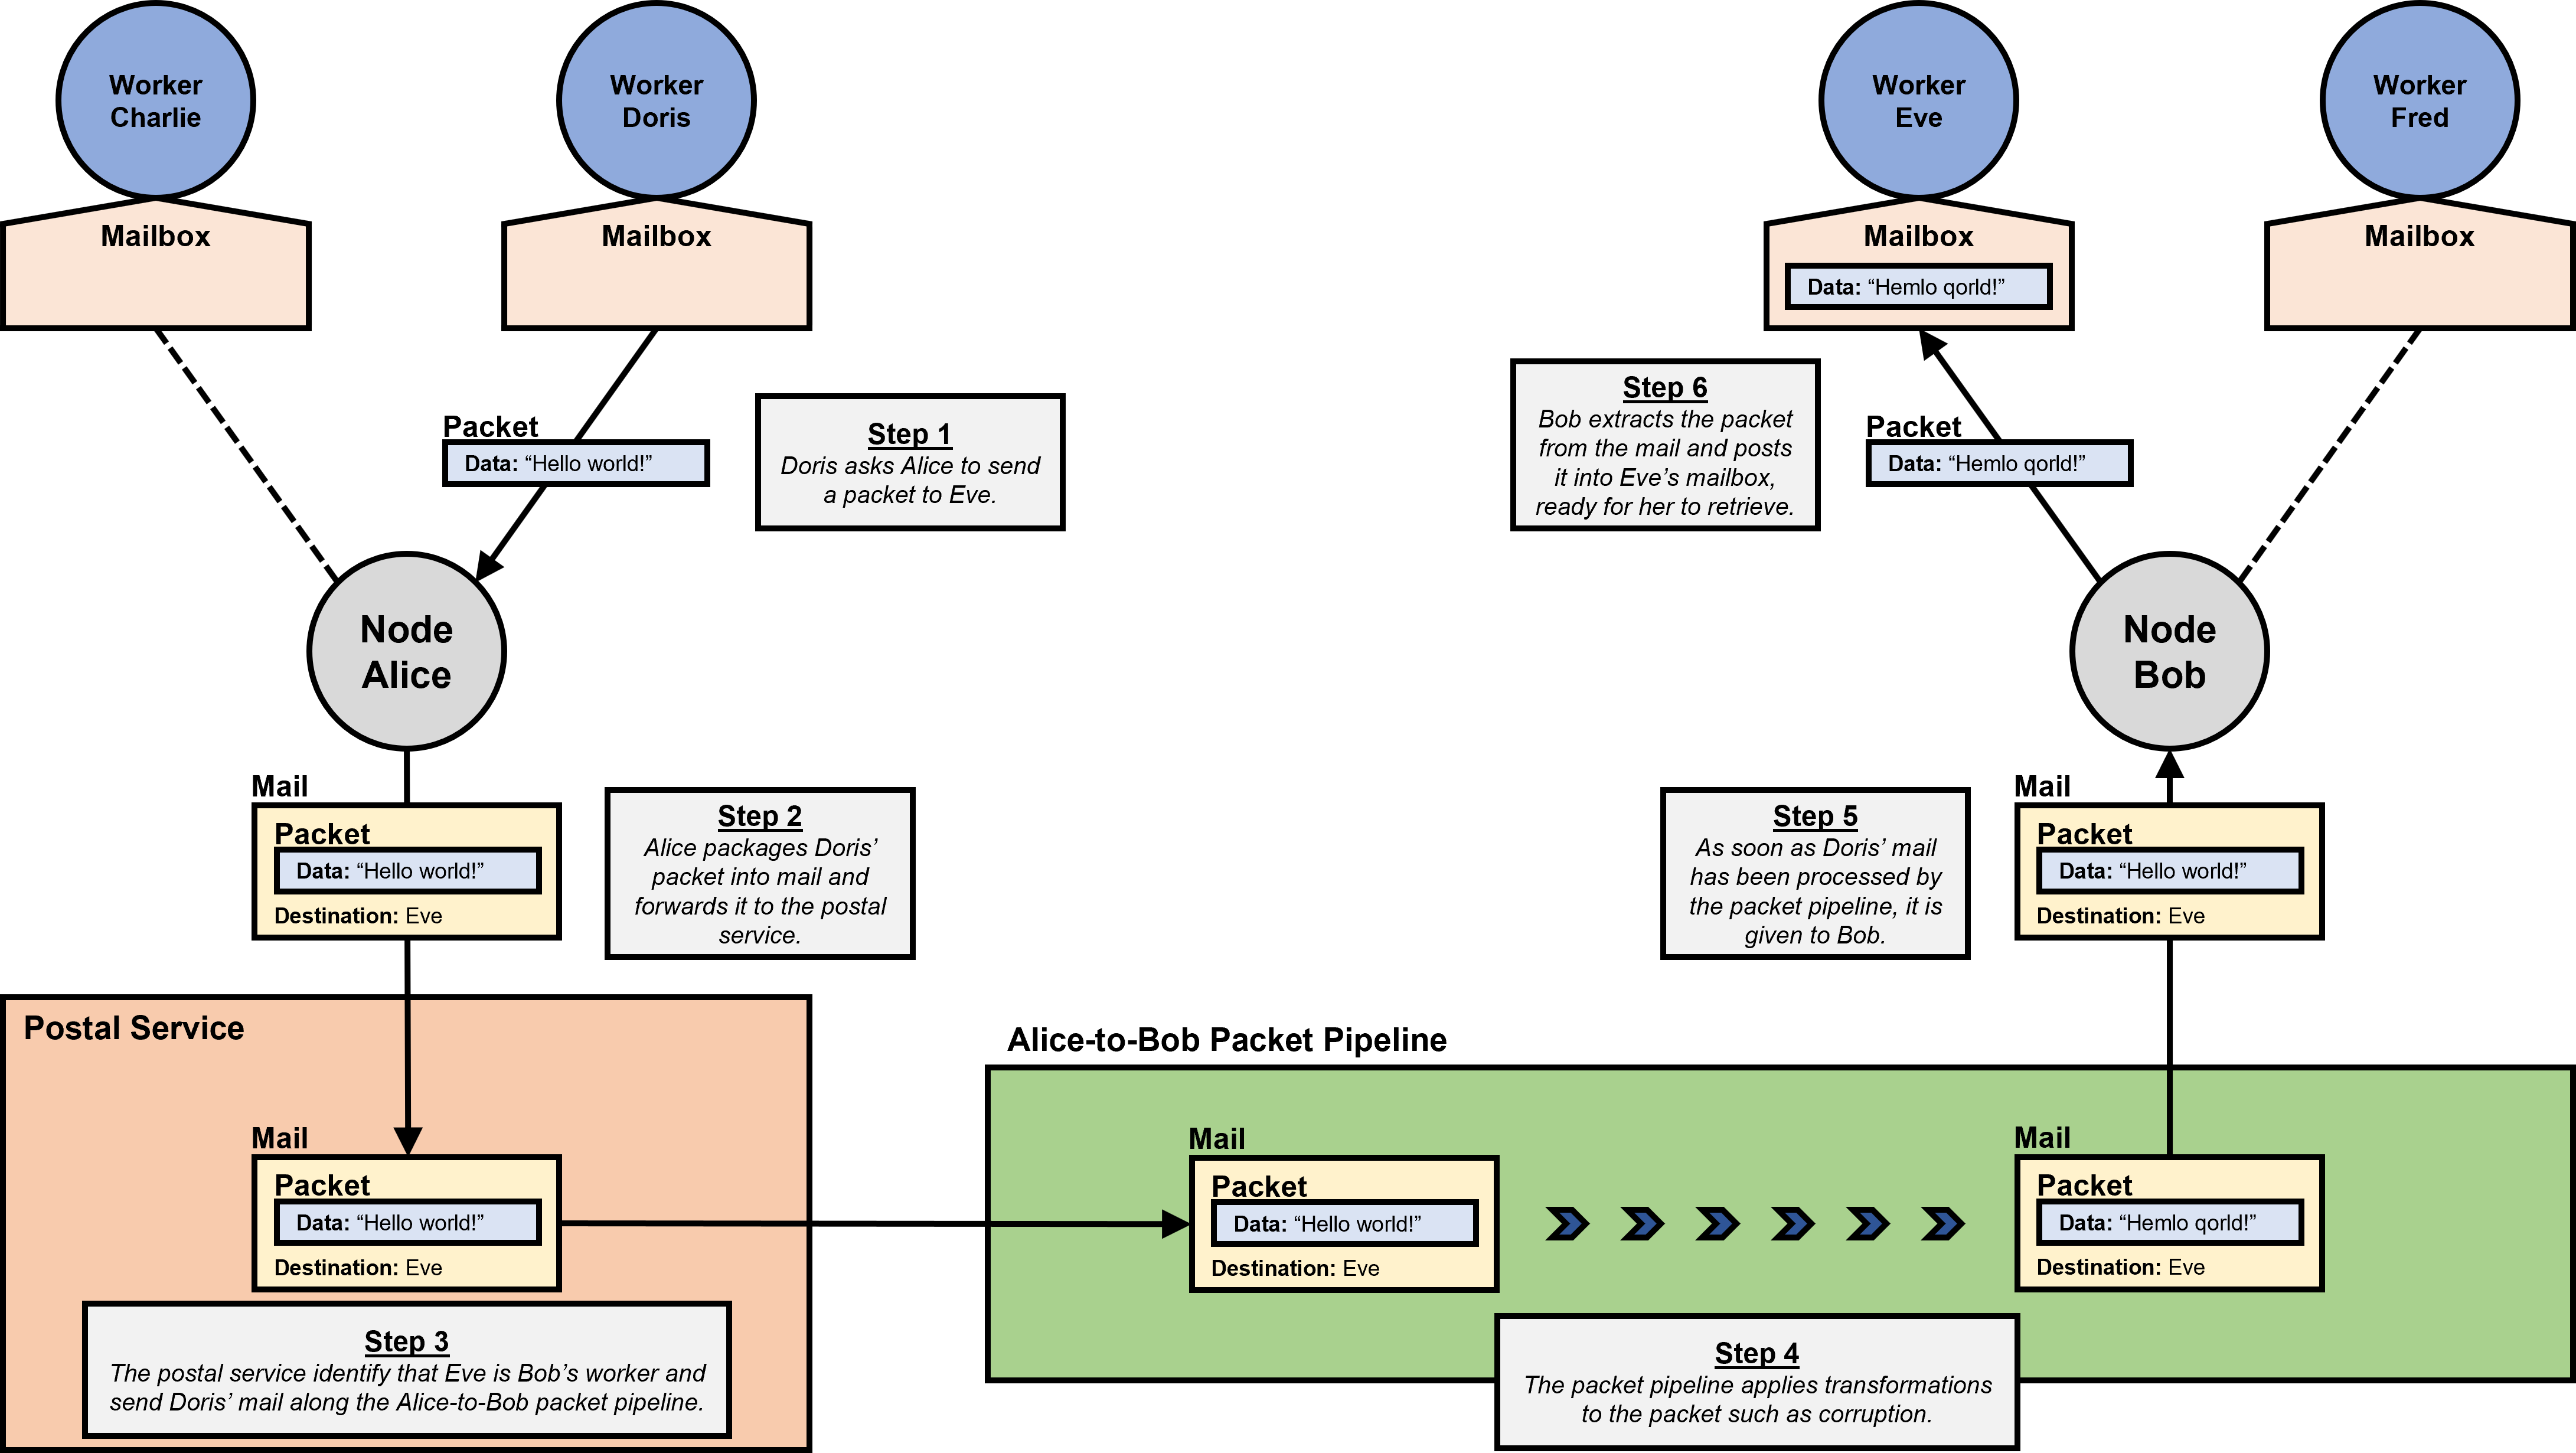
\includegraphics[width=\textwidth]{images/chapter_3_design/simulation_semantics_diagram}
    \centering
    \caption{An example of how a packet would be sent from one worker to another in a Packet Courier simulation
    .}\label{fig:chapter_3_design-simulation_semantics_diagram}
\end{figure}

In this way, workers doing work on a node can be interpreted as a group of machines being connected to a central
router. Machines can connect and disconnect freely to a router, just as workers can be spawned and killed atop a node. A
router provides each of its machines with a unique local ip-address, but has its own ip-address which it shares with
the world, just as is the case with worker and node addresses. Routers are only directly connected to their
neighbours (by definition), and as such, if a device wishes to send a message to a destination that is more than one
degree removed, then it will need to ask intermediate routers to forward the message onward. Once again, Packet
Courier is no different: nodes can only directly send mail to their immediate neighbours.

\newpage

\subsection{Network Condition Semantics}\label{subsection:network_condition_semantics}

\lettrine{W}{hen} it comes to the \emph{network} aspect of the network simulation framework that Packet Courier offers,
\texttt{tc-netem}\cite{tc_netem_wiki, tc_netem_8_man,tc_netem_src} provides an excellent template to draw from.
Indeed, Packet Courier incorporates most of the semantics that \texttt{tc-netem} lays out for itself, just with a few
subtle tweaks, namely:
\begin{itemize}
    \item \textbf{Bandwidth throttling} \\
    Constrains bitrate to a specified upper limit. \\ \\
    \emph{Packet Courier achieves this effect in a very prescriptive manner by imbuing each packet with a latency
    based on the maximum throughput and the size of the packet. For example, if the bitrate was set to 4MBps and a
    1MB packet arrived, then it would be made to wait 0.25 seconds in simulation time. This effect stacks, meaning
    that if a 2MB packet then arrived in the same tick, it would be made to wait 0.75 seconds to account for the 1MB
    of data that is yet to experience its 0.25 seconds of latency. In this way, 3MB is transferred over 0.75 seconds,
        upholding a 4MBps bitrate. \\ \\
        The general premise is to control the bitrate of a connection rather than drop excess packets. Consequently,
        packet throttling does risk becoming a black hole with respect to memory, particularly in cases where a
        high-throughput connection is being heavily throttled over a long period of time. As such, packet throttling
        should mainly be used to smooth out connections that are prone to burst behaviours, rather than as a cheap
        and dirty bitrate control mechanism. This is unlikely to satisfy users on its own, however, and as such, the
        packet throttling semantics include a drop-threshold parameter which acts as a failsafe: if the number of
        bytes currently held in the packet throttler's buffer exceeds the threshold, then incoming packets will be
        dropped until the contents of the buffer fall below this threshold again.}
    \item \textbf{Packet limiting} \\
    Enforces that only a certain number of packets can be enqueued within a certain time-frame, dropping any that
    exceed the limit. \\ \\
    \emph{Packet Courier leverages the notion of a ``packet-budget'' to decide how many packets should be enqueued
    within a particular time-frame. With each simulation tick, the time between the current simulation time and the
    last tick is measured and multiplied with the maximum number of packets per unit time to calculate the
    packet-budget, i.e.: how many packets are allowed through over the course of the next tick.}
    \item \textbf{Packet delay} \\
    Imbues packets with an artificial latency in keeping with a chosen distribution (uniform, normal or exponential).
    \\ \\
    \emph{Delay semantics are achieved by simply sampling the provided distribution and adding that value onto the
    current simulation time to produce a scheduled ``dequeue'' time. Packets can be stored in a priority queue which
    only releases the top element if the current simulation time has passed the scheduled dequeue time. \\ \\
    The only notably difference being the replacement of the Pareto distribution with the exponential distribution.
    This can be chalked up to the exponential distribution already having been implemented for other use-cases, but
    the Pareto distribution being cut due to time constraints.}
    \item \textbf{Packet drop} \\
    Samples a Bernoulli distribution and drops the packet on success. \\ \\
    \emph{Drop semantics remain the same as \texttt{tc-netem}. Gilbert Elliott and Markov modelling were left out
    because they can be replicated as part of the more general event-based semantics. ``Loss'' has been changed to
    ``drop'' to avoid confusion with notions of corruption.}
    \item \textbf{Packet corruption} \\
    Samples a Bernoulli distribution and flips a random bit on success.\\ \\
    \emph{Corruption semantics remain the same as \texttt{tc-netem}.}
    \item \textbf{Packet duplication} \\
    Samples a Poisson distribution to decide how many duplicates the given packet should have and enqueues that
    number of copies alongside the packet itself. \\ \\
    \emph{Duplication semantics remain the same as \texttt{tc-netem} with the exception that the Bernoulli distribution
    has been generalised to a Poisson distribution. Indeed, if a packet is dropped on the success of a Bernoulli
    sample with parameter $p = 0.42$, then there will be 0.42 duplicate packets on average, as would be the case with
    a Poisson distribution parameterised by $\lambda = 0.42$.}
\end{itemize}

\newpage

\subsection{Event-Based Semantics}\label{subsection:event_based_semantics}

\lettrine{I}{n} addition to simple Bernoulli sampling, \texttt{tc-netem} offers two different stateful methods to
model packet
loss\cite{tc_netem_8_man}:
\begin{itemize}
    \item \textbf{4-state Markov model} \\
    Parameters: \emph{transition probabilities $p13$, $p31$, $p32$, $p23$ and $p14$.} \\
    Semantics: \emph{``State 1 corresponds to good reception, State 4 to independent losses, State 3 to burst losses
    and State 2 to good reception within a burst.''} \\ \\
    This can be thought of more simply as a network boasting two attributes: \emph{reception} and \emph{activity}.
    Reception can either be \emph{good} or \emph{lossy}: if it is good, then packets are not dropped; if it is lossy,
    then packets are dropped. Activity can be either \emph{gap} or \emph{burst} which have no bearing on packet drop
    in isolation. Naturally these two attributes yeild a 4-state Markov model as illustrated in
    Figure~\ref{fig:chapter_3_design-tc_netem_4_state_markov_diagram}. \\ \\
    \begin{figure}[!h]
        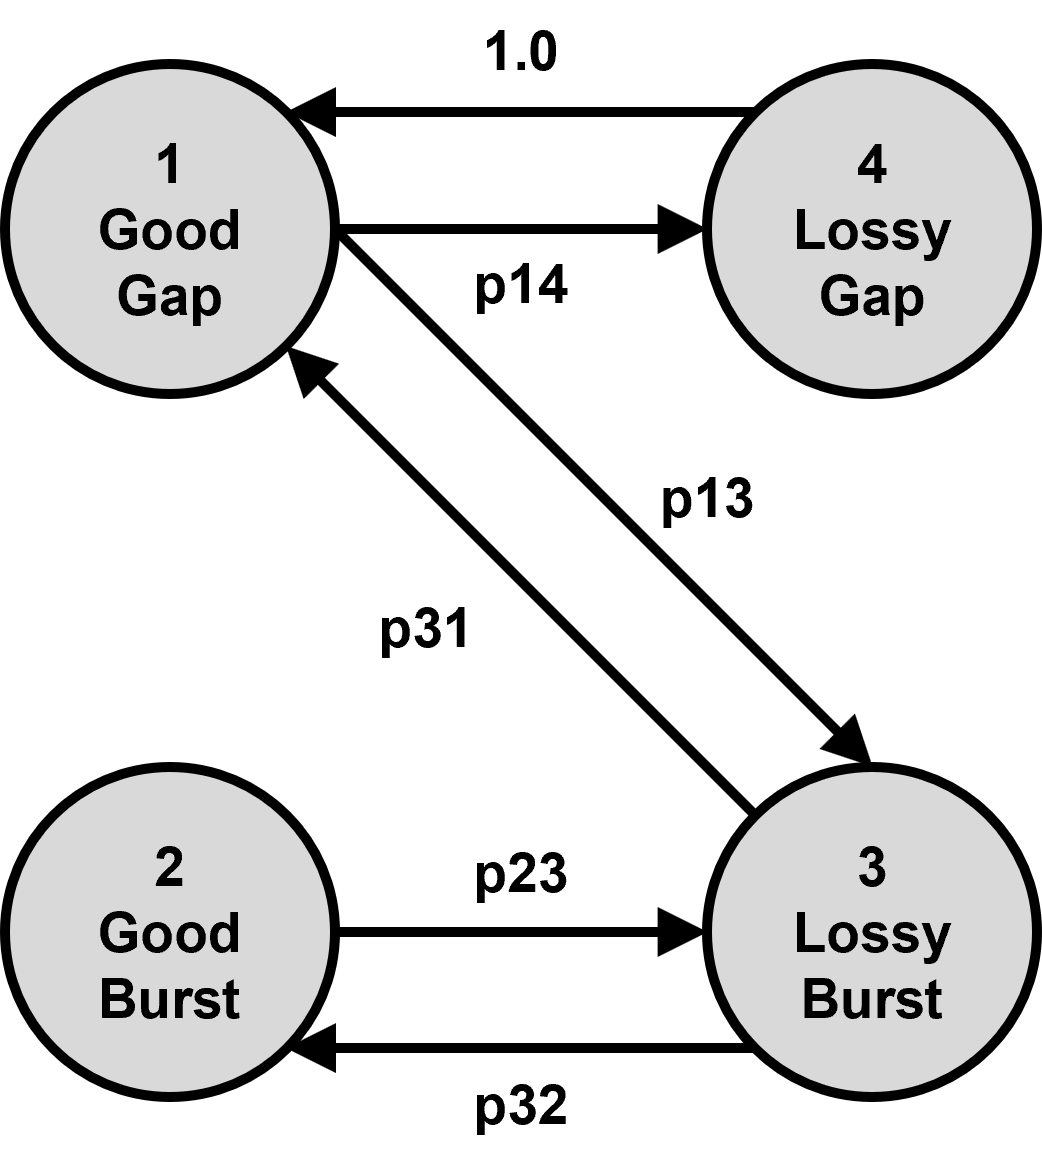
\includegraphics[width=0.35\textwidth]{images/chapter_3_design/tc_netem_4_state_markov_diagram}
        \centering
        \caption{The 4-state Markov packet loss model as implemented by
        \texttt{tc-netem}\cite{tc_netem_src}.}\label{fig:chapter_3_design-tc_netem_4_state_markov_diagram}
    \end{figure}

    The relevance of the activity attribute lies within the fact that the probability of a packet being dropped
    depends on which phase the network is currently undergoing: gap or burst.
    \item \textbf{Gilbert-Elliot loss model} \\
    Parameters: \emph{$p$, $r$, $h$ and $k$.} \\
    Semantics: \emph{``$p$ and $r$ are the transition probabilities between the bad and the good states, $1-h$ is the
    loss probability in the bad state and $1-k$ is the loss probability in the good state.''}
\end{itemize}

\newpage

Whilst these models do give users the opportunity to specify more complex packet drop conditions, they admit of the
following limitations:
\begin{itemize}
    \item \textbf{The 4-state Markov and Gilbert-Elliot models can only be applied to packet drop} \\
    If packet drop can be stateful, then it intuitively follows that other network artefacts can be as well. Indeed,
    one might ask: ``what causes a connection to enter into a `good burst' or a `lossy gap' phase?'' The answer will
    surely relate to underlying quirks of the network infrastructure, which are unlikely to affect loss of packets in
    a manner that is totally independent of latency, say. Even then, plenty of studies have shown (inadvertently or
    otherwise) that network phenomena such as delay and jitter can vary in ways that are seemingly
    stateful\cite{hpbn_mobile_networks, a_close_examination_of_4G_lte_networks,
        gsma_4G_5G_experience_evaluation_guideline, mobile_broadband_networks_under_mobility,
        emulating_3G_4G_networks, study_on_quality_of_service_in_4G_and_5G_networks,
        speed_test_russian_4G_LTE_internet_provider_Beeline}.
    Figure~\ref{fig:chapter_3_design-delay_plotted_against_time_from_study} shows one such example of this principle
    in action, whereby the latency observed appears to behave approximately according to a 3 state model: ``good'',
    where delay seems to mostly hover in the 25-30ms region; ``bad'', where delay will occassionally spike to as high
    as 50ms; ``ugly'', where delay very rarely spikes to even higher than 50ms. To illustrate this hypothesis
    further, we can see similar patterns when examining other metrics such as traffic load, as demonstrated in
    Figure~\ref{fig:chapter_3_design-traffic_load_plotted_against_time_from_study}. \\ \\

    \begin{figure}[!h]
        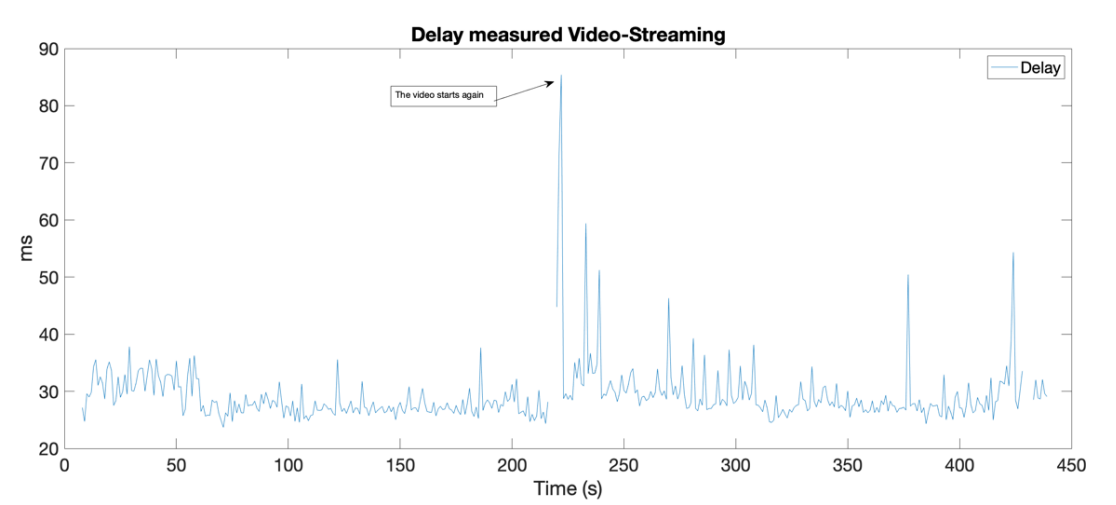
\includegraphics[width=0.9\textwidth]{images/chapter_3_design/delay_plotted_against_time_from_study}
        \centering~\caption{Delay (ms) on 4G packets bent sent as part of a video streaming service \\
        measured over time (s)\cite{study_on_quality_of_service_in_4G_and_5G_networks}.
        }\label{fig:chapter_3_design-delay_plotted_against_time_from_study}
    \end{figure}
    \begin{figure}[!h]
        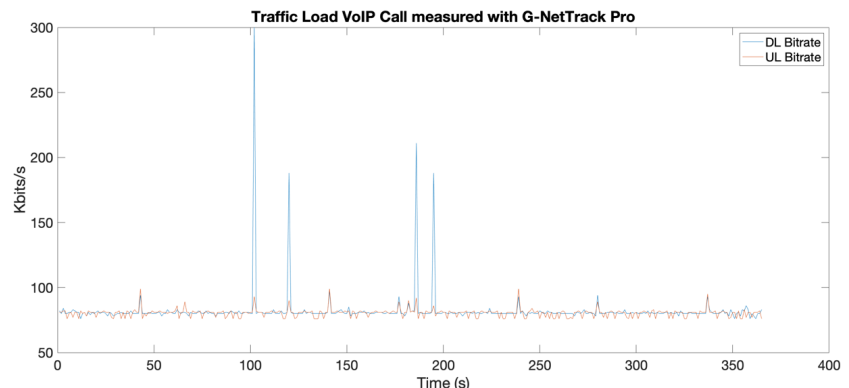
\includegraphics[width=0.9\textwidth]{images/chapter_3_design/traffic_load_plotted_against_time_from_study}
        \centering~\caption{Traffic Load (KBits/s) on 4G packets bent sent as part of a VoIP call measured over
        time (s)\cite{study_on_quality_of_service_in_4G_and_5G_networks}.
        }\label{fig:chapter_3_design-traffic_load_plotted_against_time_from_study}
    \end{figure}

    In this way, one could eyeball the number of states that would be appropriate to model the kind of conditions
    observed in Figures~\ref{fig:chapter_3_design-delay_plotted_against_time_from_study}
    and~\ref{fig:chapter_3_design-traffic_load_plotted_against_time_from_study}, only to then perform some kind of
    k-means clustering algorithm to aggregate the relevant statistics and characterise these states, i.e.: how
    frequently they occur; how long they last; how their key metric (drop, delay, traffic-load) is distributed.
    Notice that we are now in the realm of event-based semantics, where (network) events are being described by their
    interval, duration and effect, which leads nicely onto the second issue with \texttt{tc-netem}'s state-based
    models.
    \newpage
    \item \textbf{Probabilistically parameterised models are hard to reason about} \\
    Consider a network engineer who is new to a particular codebase and finds a protocol testbed with the following
    configuration:
    \begin{quote}
        \texttt{loss p13=0.5 p31=0.25 p32=0.4 p23=0.7 p14=0.15}
    \end{quote}
    There is a distinct likelihood that bafflement would ensue. \\ \\
    Although probabilistic state-based modelling can be very powerful, expressing a virtual network scenario in terms
    of state-transition probabilities does not always lend itself well to being human-readable. Most would find it
    difficult to develop a sense of how the network defined above would behave in even a coarse sense. For example,
    if packets flowed into the simulation at a constant rate, what might the graph of throughput against time look
    like? How would it be shaped? Would there be peaks and troughs, and if so, how frequently and for how long? These
    are important questions that are not necessarily self-evident from a selection of transition probabilities.
    \item \textbf{What if 4-state Markov and Gilbert-Elliot models don't fit the bill?} \\
    Unless a particular network admits of exactly one state, a ``good`` and a ``bad'' state, or four states
    characterised by ``good''/``lossy'' and ``gap''/``burst'', then it'll be a hard task to accurately model it
    using \texttt{tc-netem}. Packet loss on mobile connections has been shown to differ signicantly based on locality
    and speed of travel\cite{mobile_broadband_networks_under_mobility}, and with the gaming industry trending towards
    mobile ventures\cite{statista_mobile_gaming, rise_of_mobile_gaming}, there is a strong chance that game development
    firms will want to optimize their net-code by emulating the kind of network conditions experienced when on a
    train, bus or car journey. As such, a more general purpose set of semantics are required for undertakings of this
    nature.
\end{itemize}

\newpage

These limitations can be overcome by generalising the 4-state Markov and Gilbert-Elliot models into a discrete
event-based model\cite{discrete_event_simulation}. Packet Courier achieves this by incorperating an \emph{event
pipeline} into the core network condition semantics alongside bandwidth throttling, packet delay etc.

An event pipeline consists of a ``default'' set of network conditions and a list of possible network events.
Naturally, the default network conditions are what the pipeline will revert to when no network events are currently
underway. Network events are characterised by their mean interval and duration, as well as what network conditions
they will impose on the simulation. In instances where multiple events have been triggered at the same time, the
conditions with highest precedence will take priority. Event start and finish times are randomly generated according
to the exponential distributions $Exp(1/\mu_{interval})$ and $Exp(1/\mu_{duration})$ respectively. The
exponential distribution is not an arbitrary choice, since it is the only continuous distribution that boasts a
\emph{memoryless} property\cite{memoryless_random_variables}. Indeed, discrete event simulations are built upon
principles of memorylessness, namely because it ensures that sampled intervals and durations do not crudely depend on
the time that has already elapsed. This is crucial since events are often best modelled as being independent from one
another, insofar as an event would be scheduled in a way that is ignorant of previous events in the simulation. In a
real-world context, one can imagine a dip in 4G service being caused by a bus going underneath a bridge: would the
event of ``going under a bridge'' be described as an \emph{independent} occurrence? The answer is almost certainly
``yes''. Note however that an event pipeline is itself a network condition, so a network event could in principle
invoke a new event pipeline (only for the duration of the event, of course). This does then provide scope for
network events to ``depend'' on one another via the use of nested pipelines.

It is also no coincidence that the discrete memoryless distribution is geometric\cite{memoryless_random_variables},
not only because this is essentially the ``floored'' version of the exponential distribution, but it is used to
convert a set of state transition probabilities into discrete event parameters. Let us refer back to
Figure~\ref{fig:chapter_3_design-tc_netem_4_state_markov_diagram} as the subject for a worked example.

Let us first assume that a state transition occurs once per tick, which simply corresponds to an arbitrary unit of
time. The mean ``duration'' of each state can be computed by evaluating the expected number of consecutive ticks
without state change for each individual state. It follows that this would be distributed geometrically with the
parameter $p$ set to the probability of a state change. Hence, the mean durations for each state in
Figure~\ref{fig:chapter_3_design-tc_netem_4_state_markov_diagram} are as follows:
\begin{align*}
    \mu_{1,duration} &= \frac{1}{1 - p_{13} - p_{14}} \\
    \mu_{2,duration} &= \frac{1}{1 - p_{23}} \\
    \mu_{3,duration} &= \frac{1}{1 - p_{31} - p_{32}} \\
    \mu_{4,duration} &= 1
\end{align*}

The mean ``interval'' of each state can be similarly computed by evaluating the expected number of consecutive ticks
whereby the simulation is not in that particular state. This random variable would be distributed geometrically with
the parameter $p$ set to the probability that a state transition is not directed towards the state in question,
given that the prior state was also not the state in question. Using state 1 in
Figure~\ref{fig:chapter_3_design-tc_netem_4_state_markov_diagram} as an example, $p$ in this case would be the
probability that the simulation transitioned to state 2, 3 or 4, given that it was already in one of those states
prior. Hence, the mean intervals for each state in Figure~\ref{fig:chapter_3_design-tc_netem_4_state_markov_diagram}
are as follows:
\begin{align*}
    \mu_{1,interval} &= \frac{q_2 + q_3 + q_4}{q_2 + q_3(1 - p_{31})} \\
    \mu_{2,interval} &= \frac{q_1 + q_3 + q_4}{q_1 + q_3(1 - p_{32}) + q_4} \\
    \mu_{3,interval} &= \frac{q_1 + q_2 + q_4}{q_1(1 - p_{13}) + q_2(1 - p_{23}) + q_4} \\
    \mu_{4,interval} &= \frac{q_1 + q_2 + q_3}{q_1(1 - p_{14}) + q_2 + q_3}
\end{align*}

Where $q_i$ is the probability that the simulation is in state $i$ at any given time, which can be solved by the
following homogenous system:
\begin{align*}
    q_1 &= q_1(1 - p_{13} - p_{14}) + q_3p_{31} + q_4 \\
    q_2 &= q_2(1 - p_{32}) + q_3p_{32} \\
    q_3 &= q_1p_{13} + q_2p_{23} + q_3(1 - p_{31} - p_{32}) \\
    q_4 &= q_1p_{14}
\end{align*}

The purpose of this exercise is to illustrate the relationship between state transitional models and Packet Courier's
event-based semantics. In fact, one could generalise the above process into a set of formulaic linear equations and
hence write an algorithm to convert state transition probabilities into their respective mean durations and
intervals. This observation serves less as a proposition for a potential feature, and more a rigorous demonstration
that the semantics laid out in this section subsume the models available within the \texttt{tc-netem} framework,
converting them into a format that is more easily read and understood by humans.

\newpage

\subsection{Algorithms}\label{subsection:algorithms}

\lettrine{M}{ost} of the Packet Courier semantics as defined up until this point should map more or less directly onto a
programmed implementation. There are a few instances where this isn't the case, however, namely when sampling the
statistical distributions which sit at the heart of Packet Courier's network simulation. The normal and Poisson
distributions are particularly problematic since neither has a closed form inverse cumulative distribution function,
ergo neither can be trivially sampled by percentile.

\subsubsection{Normal Distribution Sampler}\label{subsubsection:normal_distribution_sampler}

The Box-Muller transform converts a pair of independent, uniform, random variables, $U_1, U_2 \sim U(0, 1)$ into a pair
of independent, normal, random variables $Z_0, Z_1 \sim \mathcal{N}(0, 1)$\cite{box_muller_transform} via the
following process: \\

\begin{algorithm}[caption={Box-Muller Transform\cite{box_muller_transform}.},label={alg:box_muller_transform},
    captionpos=b]
    $U_1 \gets$ sample $U(0, 1)$
    $U_2 \gets$ sample $U(0, 1)$
    $R \gets \sqrt{-2 log_e U_1}$
    $\theta \gets 2 \pi U_2$
    $Z_0 \gets R \cos \theta$
    $Z_1 \gets R \sin \theta$
\end{algorithm}

Note that this algorithm would only need to be run every other sample, since it generates two standard normal
variables. Moreover, it can be readily be adapted to any arbitrary normal distribution, since $Z \sim \mathcal{N}(0,
1) \implies \mu + \sigma Z \sim \mathcal{N}(\mu, \sigma^2)$.

\subsubsection{Poisson Distribution Sampler}\label{subsubsection:poisson_distribution_sampler}

The Poisson cumulative distribution function for $X \sim Poi(\lambda)$ as defined as follows:
\begin{align*}
    F_X(x) = e^{-\lambda} \sum_{i=0}^{\lfloor x \rfloor} \frac{\lambda^i}{i!}
\end{align*}

\begin{figure}[!h]
    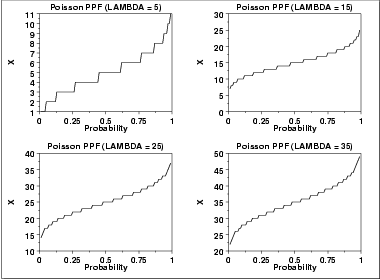
\includegraphics[width=0.9\textwidth]{images/chapter_3_design/poisson_percent_point_function}
    \centering~\caption{The inverse CDF (or PPF: percent point function) of the Poission distribution for various
        $\lambda$ parameters\cite{engineering_statistics_handbook_poisson_distribution}.}
    \label{fig:chapter_3_design-poisson_percent_point_function}
\end{figure}

As such, $F_X(x)$ sketches a step graph delimited by $x \in \mathbb{N}$ as illustrated by
Figure~\ref{fig:chapter_3_design-poisson_percent_point_function}. This property makes the Poisson distribution
perfect for tabulation, whereby the sampling strategy is to pre-compute a reasonable selection of percentile-value
pairs (i.e.: percentiles between 0 and 0.999) and perform simple lookups based on a uniform random percentile sample
$U \sim [0, 1)$.

\newpage

\begin{algorithm}[caption={Poisson distribution builder and sampler.},label={alg:poisson_builder_and_sampler},
    captionpos=b]
    function builder_poisson_table($\lambda$):
    $\quad$ $term \gets e^{-\lambda}$
    $\quad$ $percentile \gets 0$
    $\quad$ $x \gets 0$
    $\quad$ $table \gets$ new table()
    $\quad$ while $(1 - percentile) > \epsilon$ do
    $\quad$ $\quad$ add $\langle percentile, x \rangle$ to table
    $\quad$ $\quad$ $x \gets x + 1$
    $\quad$ $\quad$ $percentile \gets percentile + term$
    $\quad$ $\quad$ $term \gets term \cdot \frac{\lambda}{x}$
    $\quad$ end
    $\quad$ add  $\langle 1, x \rangle$ to table
    $\quad$ return table
    end

    function sample_poisson_table(table):
    $\quad$ $percentile \gets$ sample $U[0, 1)$
    $\quad$ $\langle lower, upper \rangle \gets$ lookup $percentile$ in table
    $\quad$ # $lower$ is the table entry where $lower.percentile$ is the
    $\quad$ # largest percentile that is smaller than the lookup parameter.
    $\quad$ # $upper$ is the converse of $lower$.
    $\quad$ # Taking $lower.x$ mimicks the flooring behaviour of $F_X(x)$.
    $\quad$ return $lower.x$
    end
\end{algorithm}


\section{Top-Down Specification}\label{section:top_down_specification}

\lettrine{N}{ow} that Packet Courier's core simulation and network semantics have been established, the next
important consideration is how this proposed functionality will be delivered to users. The path of least resistance
is to implement the framework in a way that is highly accessible for programmers to immediately interface with. From
there, more complex features can be built on top of this initial API to broaden the scope of the tool ad hoc.

\subsection{Application-Programmer Interface}\label{subsection:application_programmer_interface}

At the bare minimum, a Packet Courier simulation needs to be provided with the following parameters:
\begin{itemize}
    \item The topology of the simulated network.
    \item A set of ``scripts'' which run atop each node in the simulated network.
    \item The simulated network conditions for each node-to-node connection.
\end{itemize}

The most simple way of enabling the user to define these aspects of the simulation would be to provide them with an
API capable of the following:
\begin{itemize}
    \item Create a blank simulation configuration.
    \item Add a new, uniquely named node to a configuration.
    \item Imbue a node with a runnable ``script''.
    \item Connect two nodes with a set of network conditions.
    \item Run a configuration as a simulation.
\end{itemize}

The notion of a ``script'' which runs on each node has been quite vague thus far. The general premise would be to
spawn a root worker within each node on simulation startup, and provide them with a user defined code snippet which
will set them to work. This then presents the problem of how the user is expected to write code which interfaces with
the details of the simulation ahead of time. Alas, a worker needs to be given the autonomy to know its own address,
send packets to other workers, extract packets from its own mailbox, spawn its own child workers, etc. How can a user
take advantage of these features using a pre-programmed ``script'' that write when configuring their simulation?

Packet Courier overcomes this obstacle by modeling a \emph{Worker-Script} as a lambda that takes a
\emph{Worker-Manager} as a parameter. A worker-manager can be thought of as a collection of lambdas that together
capture the capabilities of a worker. The fact that a worker-script is a lambda allows a user to write code whilst
manipulating an arbitrary parameter which in turn provides the requisite context.
Algorithm~\ref{alg:worker_script_example} illustrates this principle in action. \\

\begin{algorithm}[caption={An example of what a worker-script might look like.},label={alg:worker_script_example},
    captionpos=b]
    function alice_worker_script(worker_manager):
    $\quad$ $neighbour \gets$ worker_manager.get_neighbour()
    $\quad$ $packet \gets$ "Hello neighbour! My name is Alice." as bytes
    $\quad$ worker_manager.send_mail($neighbour$, $packet$)
    $\quad$ $packet \gets$ worker_manager.wait_for_mail()
    $\quad$ $message \gets packet$ as string
    $\quad$ worker_manager.log($message$)
    end
\end{algorithm}

Notice that the worker-script in Algorithm~\ref{alg:worker_script_example} takes advantage of a function called
\texttt{get\_neighbour}. This then raises the question of what information should workers be provided with? Of course
they should still be provided with the basic functionality of knowing their own address, sending and receiving mail,
spawning child workers and logging messages, but what \emph{information} should they be given regarding the wider
simulation? Should they know the addresses of their neighbours? Or should they be given a blueprint of the entire
topology? How about a random subset? Should workers be able to see the current simulation time as well?

The answer to all of these questions depends on the use-case of the simulation and should ideally be decided by the
user themselves. Packet Courier achieves this using a ``care package'' style system, i.e.: a worker-manager can
provide a package of information on request, where the exact contents of this package have been defined ahead of
time by the user. This too takes advantage of a lambda called a \emph{Node-Info Generator}, which takes a snapshot of
the simulation as its parameter and processes it into a bespoke care package which workers can enjoy. This
``generation'' of node-info is only done once per node on simulation startup in case it happens to be an
intensive procedure. In this way, the call to \texttt{get\_neighbour()} on line 2 of
Algorithm~\ref{alg:worker_script_example} should in reality be something like \texttt{get\_info().get\_neighbour()}.

In summary, if a user wished to leverage this conceptual Packet Courier API, they would write some code that looked
something akin to Algorithm~\ref{alg:simulation_configuration_example}; the logged output would be:
\begin{quote}
    \texttt{> Hello neighbour! My name is Alice.} \\
    \texttt{> Greetings! I am Bob.}
\end{quote}

\newpage

\begin{algorithm}[caption={An example of what configuring a simulation might look like.},
    label={alg:simulation_configuration_example},
    captionpos=b]
    function bob_worker_script(worker_manager):
    $\quad$ $packet \gets$ worker_manager.wait_for_mail()
    $\quad$ $message \gets packet$ as string
    $\quad$ worker_manager.log($message$)
    $\quad$ $neighbour \gets$ worker_manager.get_neighbour()
    $\quad$ $packet \gets$ "Greetings! I am Bob." as bytes
    $\quad$ worker_manager.send_mail($neighbour$, $packet$)
    end

    $config \gets$ new config()
    add ("Alice" using $alice\_worker\_script$) to $config$
    add ("Bob" using $bob\_worker\_script$) to $config$
    $network\_conditions \gets$ new network_conditions()
    add (uniform packet drop from 35 to 50 in ms) to $network\_conditions$
    add ($network\_conditions$ from "Alice" to "Bob") to $config$
    add ($network\_conditions$ from "Bob" to "Alice") to $config$
    $simulation \gets$ start $config$
    wait for $simulation$ to end
\end{algorithm}

\subsection{Emulation Semantics}\label{subsection:emulation_semantics}

Although Packet Courier would be able provide value to users via APIs, it would likely alienate many developers who
were not already using the same programming language as the Packet Courier framework. Forcing prospective users to
write their simulation code in a particular language is diametrically opposed to objectives 4.b) and 5.a).

Packet Courier solves this issue by taking advantage of its own APIs to build an adaptive interface that generalises
the simulation semantics further to integrate with any arbitrary packet. Indeed, another step has been taken to
evolve the tool once more from a \emph{simulator} to an \emph{emulator}.

Imagine a game developer, Todd, who wants to test his custom networking protocol, SkyNet, for client-server
connections. Todd has built his protocol on top of UDP, since speed is more important than quality of service in the
context of hus game. Naturally, there is no real point in conducting vanilla tests on his machine, because the UDP
packets will just be internally routed by the kernel, giving Todd no understanding of how his protocol would perform
in the wild. Todd could use Packet Courier to \emph{emulate} such a scenario, but how?

Todd could leverage the simulation semantics of Packet Courier to set up a topology with two nodes, each adorning a UDP
socket. The worker at these nodes would do carry out two jobs:
\begin{itemize}
    \item Forward packets received by the UDP socket to the other worker.
    \item Send packets in the mailbox onward to the client/server via the UDP socket.
\end{itemize}

Notice however that there are now four UDP sockets in play: the client's, the server's and the two being used by
Packet Courier. As a consequence, Packet Courier needs to perform some sleight of hand here and essentially lie to
the client and the server about the ip-address of their counterpart. Thus, the client and the server will actually
end up sending their packets to Packet Courier whilst thinking that they are sending them directly to each other.

In the case where Todd wanted to test his game using multiple clients to a single server, then the exact same
principle applies. The only difference is that Packet Courier would need to keep track of which ip-addresses
corresponded to which node.

To formalise these semantics, Packet Courier is said to use an abstraction of ``public'' vs ``private'' ip-addresses in
order to slot the emulated network inbetween running processes. Each process is assigned a private ip-address which
corresponds to the address it should be sending and receiving packets on. Whilst processes could just communicate purely
using these ip-addresses, they would simply be passing messages using UDP as a protocol and the operating system
kernel as a wire; there would be no scope for manipulating the transmission of packets in a way that mimics a
particular type of internet connection.

To solve this problem, Packet Courier introduces the notion of a public ip-address, which allows Packet Courier to
intercept packets and modify them as per the user configuration. By way of analogy, one could think of a private
ip-address as a home address and a public ip-address as a PO Box. Suppose someone doesn't want mail to be sent
directly to their home for whatever reason; in this instance they can open a PO Box, whereby they collect parcels and
letters that they know are intended for them in an environment where they can be screened and processed.

\begin{figure}[!h]
    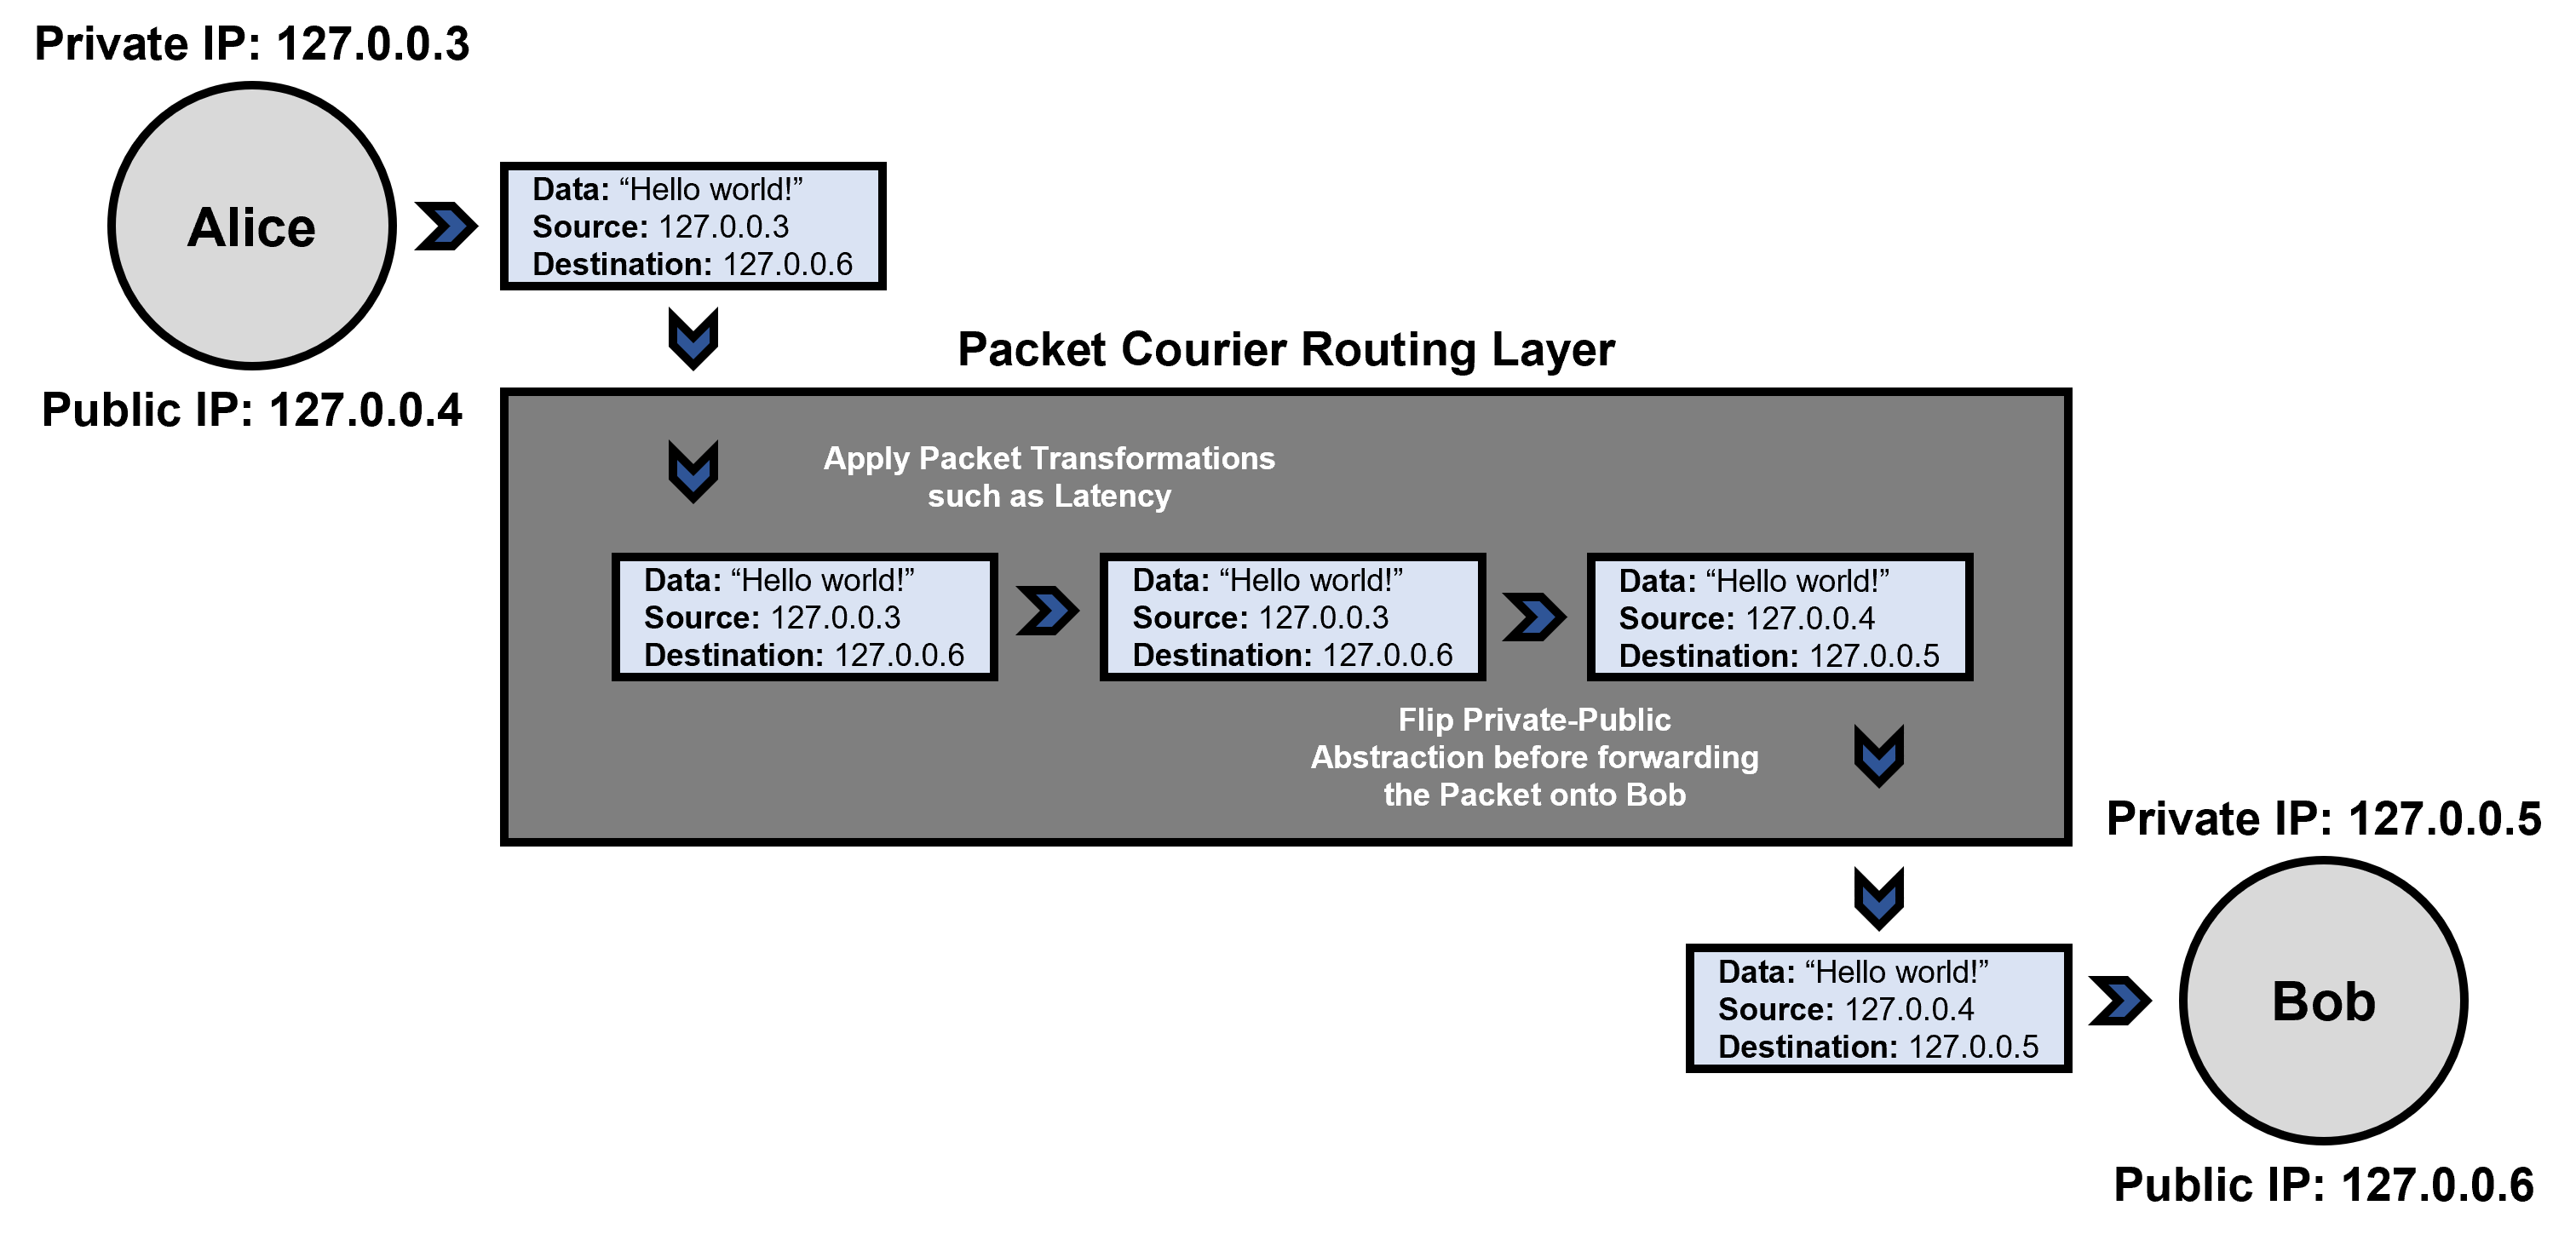
\includegraphics[width=\textwidth]{images/chapter_3_design/emulation_semantics_diagram}
    \centering~\caption{A diagram demonstrating how Alice sends a packet to Bob.}
    \label{fig:chapter_3_design-emulation_semantics_diagram}
\end{figure}

For example, consider bidirectionally connected nodes Alice and Bob (as in
Figure~\ref{fig:chapter_3_design-emulation_semantics_diagram}). Alice is told at runtime that her private ip-address is
\texttt{127.0.0.3}, her public ip-address is \texttt{127.0.0.4} and she is neighboured with Bob who has a public
ip-address of \texttt{127.0.0.6}. When Alice wants to send a packet to Bob, she should send it from her private UDP
socket with address \texttt{127.0.0.3} to the destination of \texttt{127.0.0.6}. Alice will in fact be sending her
packet to the Packet Courier routing layer, which will determine that this is Alice attempting to send a packet to
Bob, in turn applying any network conditions such as latency, loss and corruption to the packet, before forwarding it
on to Bob's private ip-address, ensuring that the source is listed as Alice's public ip-address.

One potential issue with this approach is that nodes could (accidentally or otherwise) simply pass on their private
ip-address and have other nodes bypass the emulator entirely. There is of course nothing that can realistically be
done to stop this, in the same way that there is nothing stopping users from hard coding ip-addresses into their
protocols which would have a similar effect. Ideally Packet Courier would manipulate packets at the level of the
kernel, bypassing the need for this architecture in the first place, however this just isn't very feasible in a way
that is portable, containerised and platform-agnostic. Thus, this is just a limitation that users should be
encouraged to bear in mind when using the tool.

In conclusion, Packet Courier's emulation semantics enable arbitrary processes to interface with Packet Courier
using UDP. Given that virtually every networking protocol will ultimately use UDP at the lowest-levels of
abstraction, this opens up Packet Courier to be used in real-world contexts with minimal setup. Indeed, Packet
Courier can be used as a standalone emulator and invoked from the command-line without writing a single line of
simulation code.
